\hypertarget{cart__comm_8cpp}{}\section{C\+:/\+Users/oya/\+Desktop/\+Tortoise\+S\+V\+N/\+Applications/\+Application\+\_\+\+Transporter\+Robot\+\_\+\+Vehicle/cart\+\_\+comm.cpp File Reference}
\label{cart__comm_8cpp}\index{C\+:/\+Users/oya/\+Desktop/\+Tortoise\+S\+V\+N/\+Applications/\+Application\+\_\+\+Transporter\+Robot\+\_\+\+Vehicle/cart\+\_\+comm.\+cpp@{C\+:/\+Users/oya/\+Desktop/\+Tortoise\+S\+V\+N/\+Applications/\+Application\+\_\+\+Transporter\+Robot\+\_\+\+Vehicle/cart\+\_\+comm.\+cpp}}


Function implementation for managing connections from Application\+\_\+\+Transporter\+Robot\+\_\+\+Cart processes. ~\newline
.  


{\ttfamily \#include \char`\"{}cart\+\_\+comm.\+h\char`\"{}}\newline
{\ttfamily \#include \char`\"{}cart\+\_\+status\+\_\+copy.\+h\char`\"{}}\newline
{\ttfamily \#include \char`\"{}ulapi.\+h\char`\"{}}\newline
{\ttfamily \#include $<$string$>$}\newline
{\ttfamily \#include $<$stdio.\+h$>$}\newline
{\ttfamily \#include $<$stdlib.\+h$>$}\newline
{\ttfamily \#include $<$iostream$>$}\newline
Include dependency graph for cart\+\_\+comm.\+cpp\+:\nopagebreak
\begin{figure}[H]
\begin{center}
\leavevmode
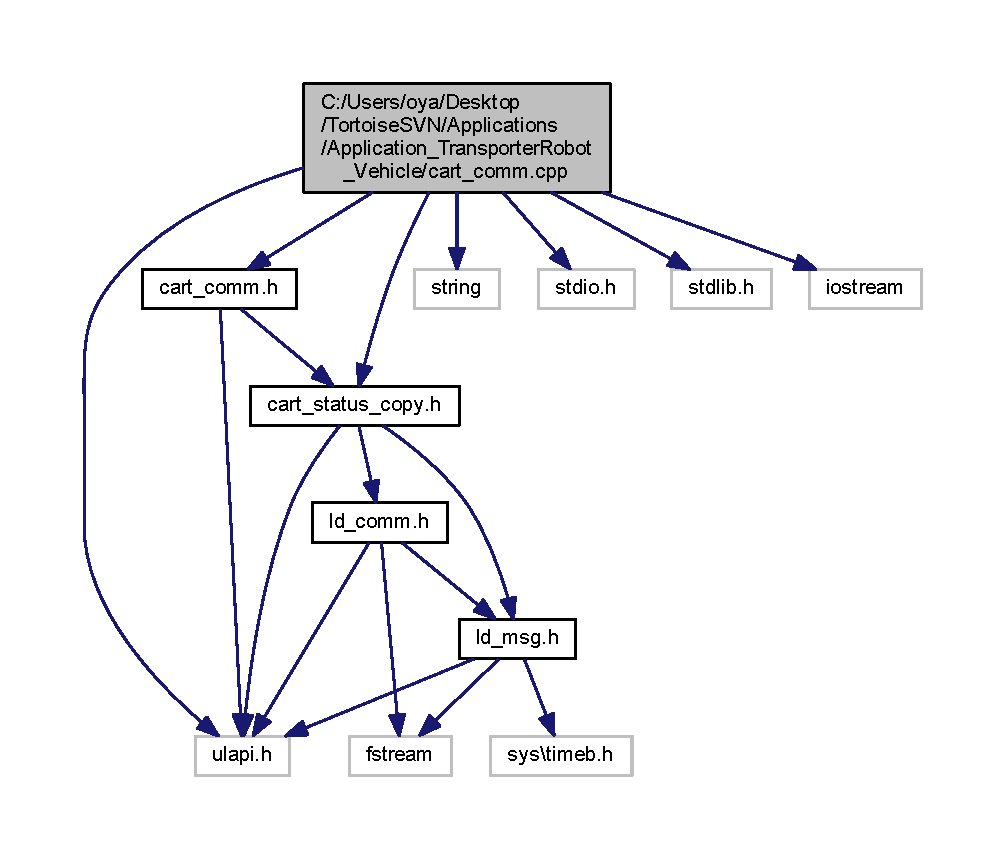
\includegraphics[width=350pt]{cart__comm_8cpp__incl}
\end{center}
\end{figure}


\subsection{Detailed Description}
Function implementation for managing connections from Application\+\_\+\+Transporter\+Robot\+\_\+\+Cart processes. ~\newline
. 

References\+: ~\newline
 Based on\+: lynx\+\_\+comm.\+h by O. Aboul-\/\+Enein ~\newline
 \mbox{[}1\mbox{]} Beginning Linux Programming, Chapter 15, Neil Matthew and Richard Stones ~\newline
\mbox{[}2\mbox{]} stackoverflow.\+com/questions/11842416/function-\/does-\/not-\/change-\/passed-\/pointer-\/c ~\newline
\mbox{[}3\mbox{]} stackoverflow.\+com/questions/13818960/c-\/tcp-\/server-\/still-\/reading-\/data-\/after-\/client-\/disconnects ~\newline
(S\+O\+L\+U\+T\+I\+ON TO B\+L\+O\+C\+K\+I\+NG S\+O\+C\+K\+ET P\+R\+O\+B\+L\+EM, you need to check for a return value of 0 since a 0 return values means client disconnected! ~\newline
your loop does not check for zero so it repeats the read call)

\begin{DoxyAuthor}{Author}
Omar Aboul-\/\+Enein 
\end{DoxyAuthor}
\begin{DoxyDate}{Date}
2017-\/06-\/05 
\end{DoxyDate}
